\documentclass{article}
\usepackage{tikz}
\begin{document}
 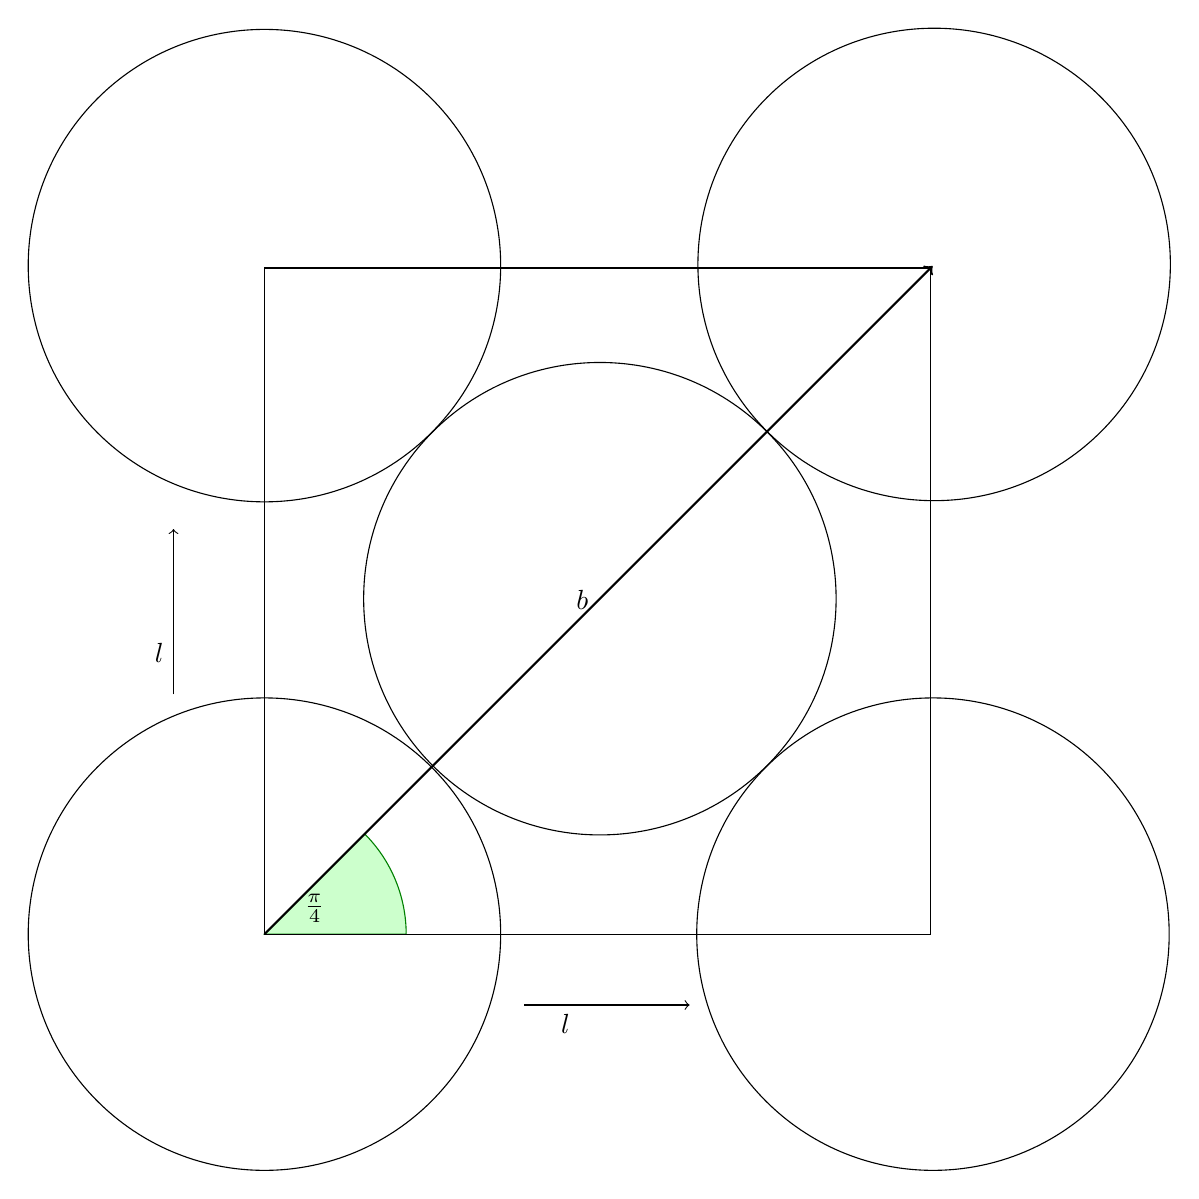
\begin{tikzpicture}[scale=3]
 %\draw[step=.5cm, gray, very thin] (-1.2,-1.2) grid (1.2,1.2); 
\filldraw[fill=green!20,draw=green!50!black] (0,0) -- (6mm,0mm) arc (0:45:6mm) -- cycle node[midway, below]{$\frac{\pi}{4}$}; 
 \draw(0,0) -- (2.82,0) coordinate (x axis);
 \draw (0,0) -- (0,2.82) coordinate (y axis) ;
  \draw  (2.82,0) -- (2.82,2.82) coordinate (y axis);
   \draw (0,2.82) -- (2.82,2.82) coordinate (y axis);
      \draw[->] (1.1,-.3) -- (1.8,-.3)  coordinate (y axis) node[near start,below] {$l$ } ;
      \draw[->] (0,1.4,) -- (0,2.1 ,)  coordinate (y axis) node[near start,left] {$l$ } ;

 \draw (0,0) circle (1cm);
 \draw (1.42,1.42) circle (1cm);
 \draw (2.835,2.835) circle (1cm);
  \draw (0,2.83) circle (1cm);
   \draw (2.83,0) circle (1cm);


 %\draw[very thick,red] (45:1cm) -- node[left,fill=white] {$\sin \alpha$} (45:1cm |- x axis);
 %\draw[very thick,blue] (45:1cm |- x axis) -- node[below=2pt,fill=white] {} (0,0);
 \draw[->, thick] (0,0) -- (45:4cm) node[midway,left] {$b$ };
 %\foreach \x/\xtext in {-1, -0.5/-\frac{1}{2}, 1} 
 %  \draw (\x cm,1pt) -- (\x cm,-1pt) node[anchor=north,fill=white] {$\xtext$};
 %\foreach \y/\ytext in {-1, -0.5/-\frac{1}{2}, 0.5/\frac{1}{2}, 1} 
 %  \draw (1pt,\y cm) -- (-1pt,\y cm) node[anchor=east,fill=white] {$\ytext$};
 \end{tikzpicture}
 
 
\end{document}